%======================================================================
\chapter{Modeling in CoppeliaSim}
\label{ch: coppSimModeling}
%======================================================================

%----------------------------------------------------------------------
\section{Problem Statement}
%----------------------------------------------------------------------
It is important to be able to simulate a robot's behavior before using the
actual robot to help find unexpected behaviors. CoppeliaSim is commercial robot
simulation software with the ability to simulate a robot that would operate in
exactly the way it would happen with a real robot. However, the robot of
interest is not currently included in CoppeliaSim's library that leads to
creating a model of the robot and simulating it before practical implementation.
The following sections explain how to model the Runt Rover robot in CoppeliaSim.

%----------------------------------------------------------------------
\section{Dimensions and 3D Modeling}
%----------------------------------------------------------------------
The Runt Rover robot is geometrically simple, with only a few dimensions being necessary to model the shape of the body and wheels. The dimensions used in this guide are shown in Fig. \ref{fig:runtRoverDims}

\begin{figure}
    \centering
    
\includegraphics[width=3.5in]{figs/img/runtRoverDimensions}
    \caption{Dimensions of the Runt Rover Robot}
    \label{fig:runtRoverDims}
\end{figure}

The final 3D models are shown in Fig. \ref{fig:runtRoverModels}. An arrow was placed on the body to indicate orientation during simulation.

\begin{figure}
    \centering
    \begin{subfigure}[b]{0.6\textwidth}
        \centering
        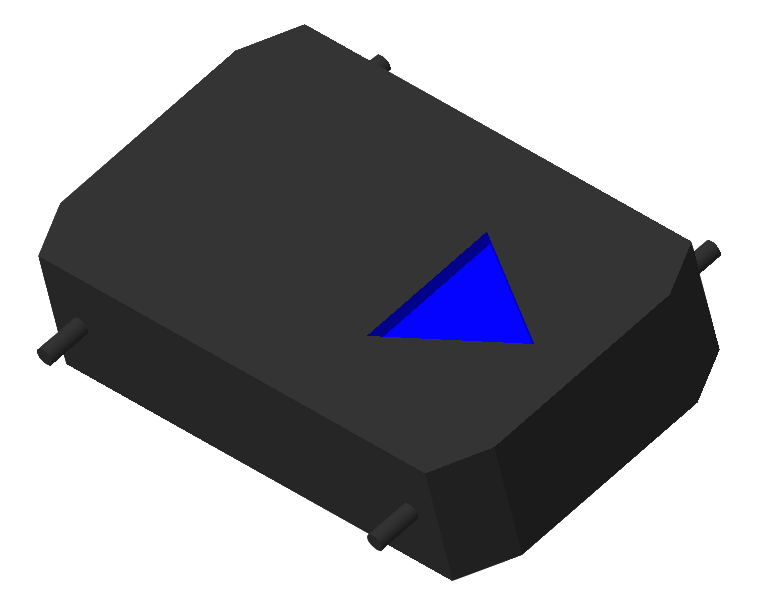
\includegraphics[width=\textwidth]{figs/img/runtRoverChassis}
        \caption{Chassis}
        \label{fig:runtRoverChassis}
    \end{subfigure}
    \hfill
    \begin{subfigure}[b]{0.3\textwidth}
        \centering
        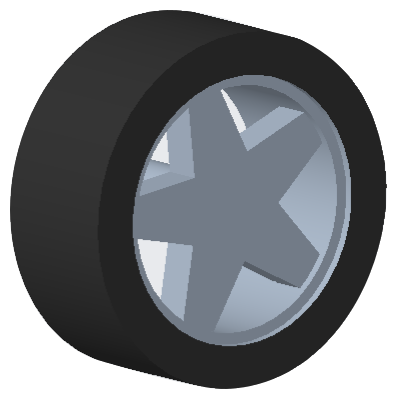
\includegraphics[width=\textwidth]{figs/img/runtRoverWheel}
        \caption{Wheel}
        \label{fig:runtRoverWheel}
    \end{subfigure}
    \caption{Modeled Parts}
    \label{fig:runtRoverModels}
\end{figure}

%----------------------------------------------------------------------
\section{Importing Models}
%----------------------------------------------------------------------
The next step is to import the 3D models into CoppeliaSim. This is accomplished using File \textgreater \ Import \textgreater \ Mesh. If the models were dimensioned in millimeters, the scale must be changed to 0.001 since CoppeliaSim uses meters. Since there are multiple colors in the models, there will be multiple shapes in CoppeliaSim. These can be grouped by dragging one shape onto another. Also, the shapes can be renamed. In modeling the Runt Rover, one chassis and four wheels are needed. The wheels must be placed in the correct locations on the axles.

%----------------------------------------------------------------------
\section{Adding Motors}
%----------------------------------------------------------------------
The robot can be given motors by means of revolute joints. These can be added using Add \textgreater \ Joint \textgreater \ Revolute. For the Runt Rover, one revolute joint was placed at each wheel. The joints should be named according to the wheel location since their names are used to interface the robot with Matlab. These joints are then made invisible by moving them to visibility layer 10. This is achieved in the Object Common Properties dialog box. The joints can be viewed by turning on visibility for layer 10 using the Layers dialog box. In the Object Properties dialog box, there is a button to open the Dynamic Properties dialog box. In this box, make sure the ``Motor enabled'' checkbox is enabled.

%----------------------------------------------------------------------
\section{Dynamic Shapes}
%----------------------------------------------------------------------
The 3D models do not have any dynamic properties within CoppeliaSim. It is recommended to use primitive shapes for the dynamic properties to reduce computation during simulation. For the Runt Rover, the wheels can be dynamically represented as cylinders, and the chassis can be dynamically represented as a cuboid. To add a primitive cylinder, use Add \textgreater \ Primitive Shape \textgreater \ Cylinder, and specify the size to be the same as a wheel. To add a cuboid, use Add \textgreater \ Primitive Shape \textgreater \ Cuboid, and specify the size to be the same as the chassis. These bodies must now be configured with the appropriate dynamic properties.

In the dynamic properties dialog box, make sure the ``Body is respondable'' checkbox is enabled, and enable the first four checkboxes and disable the last four checkboxes in the local respondable mask. Repeat this process on all of the dynamic shapes, alternating between selecting the first four and selecting the last four checkboxes in the local respondable mask. To give the robot mass and inertia, make sure the ``Body is dynamic'' checkbox is enabled, and click the ``Compute mass and inertia'' button. These dynamic shapes should be named according to the parts they represent (FrontLeftWheelDyn, for example). In the Object Common Properties dialog box, assign the dynamic shapes to visibility layer 9 to make them invisible.

%----------------------------------------------------------------------
\section{Linkage}
%----------------------------------------------------------------------
Now it is time to link everything together into one robot. First assign each graphical shape to its corresponding dynamic shape by dragging and dropping it onto the dynamic shape. Then assign the dynamic shapes for the wheels to the corresponding revolute joints in the same way. Finally, assign the revolute joints to the dynamic chassis. The name of the dynamic chassis is the name that will be used to interface with Matlab, so change it to ``RuntRover.'' Assign this shape to be the model base in the Object Common Properties dialog box. To make the bounding box the correct size, select the revolute joints and enable the ``Ignored by model bounding box'' and the ``Invisible during selection'' checkboxes in the Object Common Properties dialog box. Now enable the ``Select base of model instead'' checkbox for each of the visible objects. This allows us to select the entire robot by clicking on any part.

%----------------------------------------------------------------------
\section{Saving the Model}
%----------------------------------------------------------------------
To save this model, go to File \textgreater \ Save model as \textgreater \ CoppeliaSim model. The default location should be in the CoppeliaSim models directory. Create a new directory to contain your models and save the model within that directory. Your model will now be available in the CoppeliaSim library.


%%% Local Variables:
%%% mode: latex
%%% TeX-master: "../finalReport"
%%% End:
